\chapter{Modelling}
\label{ch:modelling}
After explaining thermal basics and the electrical analogy, these foundations are used in this chapter. The development process and the results of the thermal model of the reference building will be presented. Later, the model is needed for the MPC to predict the thermal reactions of the building.
\newline
    
    The focus of this work is on the MPC part, so a simple thermal model is required. Nevertheless, no necessary information should be missing: (i) the thermal storage possibilities, (ii) the temperature inside of the building, and (iii) the influence of the heating system. The storage allows heating while the grid has too much power and saving energy in the building, while the grid requires power. This behaviour is necessary to achieve the MPC's goal of providing grid services. The output of the model must be the inside temperature, as customer comfort is controlled by the air temperature using the MPC. Finally, the influence of the heating system must be visible in the model, as it is the input of the system.
    \newline
    The thermal model reflects the thermal conditions of the reference building. Therefore, the inner energy of the water reservoir and the air temperature inside the building are modelled. The water reservoir and the building behaviour are modelled according to different modelling strategies. The following chapters describe the submodels water reservoir and building model, the kind of modelling, and the conclusion of the submodels.
    
    \section{The modelling strategies}
    \label{ModellingStrategies}
    There are three types of modelling strategies to derive building models the so-called white-box models, grey-box models or black-box models. White-box models describe the system in terms of first principles from physics. Black-box models, on the other hand, have no physical description. They are created from data. And grey-box models are in between these two options \cite{Statusseminar.ForschungfurEnergieoptimiertesBauen.2009}. All approaches are used in the thermal modelling of buildings \cite{Kramer.2012}.
    \newline
    The chosen approach for the MPC is the \textbf{grey-box model} for two reasons: First, this approach combines the advantages of white-box models and black-box models \cite{EstradaFlores.2006}. Second, there is the possibility to generate the required data from the reference building with the available measurement equipment at KIT. According to Coakley et al., further advantages and disadvantages are among other things \cite{Coakley.2014}:
    \begin{table}[h!]
    \label{Advantages and disadvantages of grey-box modelling}
        \centering
        \begin{tabular}{p{7.3cm} | p{7.3cm}}
        \hline
          Advantages  &  Disadvantages\\
        \hline
        \begin{itemize}
            \item faster development by a combination of physical and statistical model
        \end{itemize}
      & \begin{itemize}
            \item requires knowledge in physical and statistical modelling 
        \end{itemize}\\
     \begin{itemize}
            \item accuracy of the results for the specific use case, provided by qualitative training data
        \end{itemize} & \begin{itemize}
            \item changes at the building lead to a re-training
        \end{itemize}\\
        \end{tabular}
        \caption {Advantages and disadvantages of grey-box modelling}
    \end{table}
    \newline
    However, the water reservoir and the heating system are not in use, yet. So, no data is available for training a grey-box model. Thus, this submodel needs to be designed as a \textbf{white-box model}.
    \newline
    The benefits and challenges of white-box models are presented in \autoref{tab:wihte-boxpro} \cite{EstradaFlores.2006}.
    \begin{table}[h!]
        \centering
        \begin{tabular}{p{7.3cm} | p{7.3cm}}
        \hline
          Advantages  &  Disadvantages\\
        \hline
        \begin{itemize}
            \item relies on physics
        \end{itemize}
      & \begin{itemize}
            \item necessitate assumptions for simplification
        \end{itemize}\\
     \begin{itemize}
            \item applicable for every situation with the same assumptions and requirements 
        \end{itemize} & \begin{itemize}
            \item commonly complex mathematical solution methods
        \end{itemize}\\
        \end{tabular}
        \caption {Advantages and disadvantages of white-box modelling}
        \label{tab:wihte-boxpro}
    \end{table}

    \section{The water reservoir model}
    \label{waterModel}
    For the modelling of the water reservoir (WR) \nomenclature[A]{WR}{Water Reservoir}, all heat flows that influence the water reservoir are considered (see \autoref{fig:Figure of the water reservoir with the heat flows}). The heat pump (HP) \nomenclature[A]{HP}{Heat Pump} feeds the water reservoir with heat flow $\dot{Q}_\text{HP}$. The service water (SW) \nomenclature[A]{SW}{Service Water} and the water for the heating circuit are removed from the storage. Since no service water is currently connected to the reference building, the heat flow $\dot{Q}_\text{SW}$ will be set to zero in the following. The heat losses $\dot{Q}_\text{loss}$ and the heating heat flow  $\dot{Q}_\text{heating}$ are the discharged heat flows. The resulting energy balance according to \autoref{eq:1HS} reads:
    \begin{equation}
        \label{waterReservoir}
        \frac{d U_\text{WR}}{d t}= -\dot{Q}_\text{heating} + \dot{Q}_\text{HP} - \dot{Q}_\text{loss}
    \end{equation}
    
    \begin{figure}[H]
        \centering
        \def\svgwidth{120pt}
        \input{figure/Wasserspeicher.pdf_tex}
        \caption{Illustration of the water reservoir with the heat flows}
        \label{fig:Figure of the water reservoir with the heat flows}
    \end{figure}
    Since the model is based on a real building, the size of the heat flows and the inner energy are limited according to the devices of the building, e.g. the heat pump. Further, we have to consider that the heat flows $\dot{Q}_\text{HP}$ and $\dot{Q}_\text{heating}$ can also have negative values when cooling is required. The heat losses and the heat pump heat range are taken from the technical data \cite{Oskar}, \cite{TUM}.\newline
    Since the reference water reservoir is stratified storage we determine the maximum inner energy under the assumption of two heat layers. According to \autoref{eq:innerEnergy}, we need material parameters of water ($c_\text{v,w}$, $\rho_\text{w}$), the size of the water reservoir ($m = \rho_\text{w} V$), both are known, and a temperature difference, which we define for both layers. To determine the temperature difference, we define two temperatures at the time one and two. At the time one, we assume that the storage has ambient temperature $T_\text{amb}$ of 20°C in both layers. At the time two, we differentiate the temperatures in the layers. The maximum temperature of the upper layer in the water reservoir $T_\text{max,1}$ is the maximum inlet temperature of 55 °C of the heat pump provided by the characteristic diagram. The maximum temperature of the lower layer $T_\text{max,2}$ is based on the inlet temperature of the underfloor heating at 35 °C. We calculate the sum of the inner energy as follows.
    \begin{equation}
        \label{eq:max.Energie}
        U = \rho_\text{w} c_\text{v,w} ((T_\text{max,1}-T_\text{amb})\cdot \frac{V}{2} + (T_\text{max,2}-T_\text{amb})\cdot \frac{V}{2}) 
    \end{equation}

    \section{The building model}
    \label{sec:building model}
    First, the thermal dynamics of the building must be described physically. To comply with the requirement of a simple model, we model the building as a single zone, as often practised in the literature \cite{Park.2011}, \cite{Hazyuk.2012}. Single zone means that we average the values of interest of the rooms, such as air temperature or wall temperature to one representative value for the entire building. 
    \newline
    We consider the air temperature, the temperature of the outer walls, the temperature of the inner walls and floors in the first floor, and the temperature of the floor in the model. In the following, these temperatures are called: inside temperature  $T_\text{inside}$, envelope temperature $T_\text{envelope}$, interior temperature $T_\text{interior}$, and floor temperature $T_\text{floor}$. 
    Using the state-space formulation (see \autoref{subsection:dynamics}), the temperatures are states in this model. According to the RC-analogy (see \autoref{electricalanalogy}), the model is built and explained in more detail in the following for every state. \newline
    
    \textbf{Inside temperature:}\newline
    The inside temperature $T_\text{inside}$ is the main parameter in the model because we control it in the MPC. To generate high accuracy the impacts on $T_\text{inside}$ are modelled more specific. Therefore, compared to the description of the other states, a more precise description of the dynamics of the inside temperature is required. We consider the influence of the sun $\dot{Q}_\text{sun,inside}$, the heating system $\dot{Q}_\text{heating}$ and the other states in the way shown in the following equation. $\dot{Q}_\text{heating}$ links the water reservoir model and the building model as the flow from the reservoir to the building. 
    \begin{align}
        \label{eq:1.state}
        C_\text{inside}\cdot \frac{d T_\text{inside}}{d t} &=& \dot{Q}_\text{heating} + \dot{Q}_\text{sun,inside} - \frac{T_\text{inside}-T_\text{envelope}}{R_\text{inside}} - \frac{T_\text{inside}-T_\text{outside}}{R_\text{window}} \\
       & &-\frac{T_\text{inside}-T_\text{interior}}{R_\text{interior}}-\frac{T_\text{inside}-T_\text{floor}}{R_\text{floor}}\nonumber
    \end{align}
    The detailed explanation for the composition of the thermal resistance and capacitance is in \autoref{electricalanalogy}. In the following table, the material and state dependant values are explained:
    \begin{table}[H]
        \centering
        \begin{tabular}{l p{13cm}}
            $C_\text{inside}$ & The thermal capacitance $C_\text{inside}$ is calculated from the mass of the air from all rooms and the heat capacity of the air (1006 $J/(kg K)$ \cite{Weigand.2016}). The mass can be determined with the volume of the rooms according to the construction plan \cite{Bauplan} and the air density (1.28 $kg/m^3$ \cite{Weigand.2016}).\\
            $R_\text{inside}$ & The thermal resistance $R_\text{inside}$ includes a convective part with the transfer coefficient $\alpha = 0.9 W/(m^2 K)$ for air perpendicular to the wall in buildings with the assumption of one Kelvin temperature difference between the wall and air \cite{Schweizer-fnalpha}.\\
            $R_\text{window}$ & The window resistance $R_\text{window}$ is determined with the window area and the assumption of a heat transmission coefficient $u = 1 W/(m^2 K)$ \cite{ThorbenFrahm.2021}.\\
            $R_\text{floor}$ & Heat conductivity and heat convection are the regarded mechanisms to determine the floor resistance $R_\text{floor}$. The floor material is reinforced concrete with the thermal conductivity of $2.3 W/(m K)$ \cite{AntonSchweizer.12.10.2021}.\\
            $R_\text{inside}$ & For the convection inside the building, the same assumptions are made as for $R_\text{inside}$.\\
            $R_\text{interior}$ & The interior resistance $R_\text{interior}$ is also calculated with the heat transfer coefficient inside.
        \end{tabular}
        \caption{Explanation of the special material and state dependant values of the differential equation of the inside temperature}
        \label{tab:valuesOfInsideTemperature}
    \end{table}
    
    \textbf{Envelope Temperature:}\newline
    The envelope temperature is influenced by the sun, the contact of the walls with the inner air temperature and with the outside temperature. The sun affects the air temperature differently than the outer walls. Therefore, we differentiate between the influence of the sun on the inner air temperature and the envelope, and we consider here $\dot{Q}_\text{sun,envelope}$ in the opposite to \autoref{eq:1.state} considering $\dot{Q}_\text{sun,inside}$.
    \begin{equation}
    \label{eq:diffEnvelope}
        C_\text{envelope}\cdot \frac{d T_\text{envelope}}{d t} = \dot{Q}_\text{sun,envelope} - \frac{T_\text{envelope}-T_\text{outside}}{R_\text{envelope}} + \frac{T_\text{inside}-T_\text{envelope}}{R_\text{inside}}
    \end{equation}
    \begin{table}[H]
        \centering
        \begin{tabular}{l p{13cm}}
        $R_\text{envelope}$ & The outer wall resistance $R_\text{envelope}$ contains a heat conductivity of aerated concrete ($0,133 W/(m K)$ \cite{GhaziWakili.2015}) and the heat transfer coefficient for air perpendicular to the wall outside $\alpha_\text{envelope}$ according to the rules of thumb from Schweizer-fn $\alpha_\text{envelope} = 3.96 (v / L)^{0.5} = 1.669 W/(m^2 K)$ \cite{Schweizer-fnalpha} with the average wind velocity of Karlsruhe $v$ \cite{AbteilungKlimaundUmweltberatung.2004} and the length of the building wall.\\
        $C_\text{envelope}$ & To determine the capacitance $C_\text{envelope}$, we need the volume of the outer walls from the construction plan \cite{Bauplan}, the density of aerated concrete ($485 kg/m^3$) and the capacity (1000 $J/(kg K)$) \cite{GhaziWakili.2015}. 
        \end{tabular}
        \caption{Explanation of the special material and state dependant values of the differential equation of the envelope temperature}
        \label{tab:valuesOfEnvelopeTemperature}
    \end{table}
   
    \textbf{Interior and floor temperature:}\newline
    The differential equations for the interior and the floor temperature only interact with the inside temperature. 
    Hazyuk et al. \cite{Hazyuk.2012} models also the ground floor as one state. The explanation is that the ground floor has no convective contact with the environment. Therefore, the ground floor is not modelled with the envelope for receiving the correct physical description, where the wind has an impact on the outer walls.
    The interior is modelled to improve the accuracy of the inside temperature equations because of the special consideration of the capacitance of the inner walls.
    \begin{align}
    C_\text{interior}\cdot \frac{d T_\text{interior}}{d t} &= \frac{T_\text{inside}-T_\text{interior}}{R_\text{interior}} \\
       C_\text{floor} \cdot \frac{d T_\text{floor}}{d t} &= \frac{T_\text{inside}-T_\text{floor}}{R_\text{floor}} \nonumber\\
    \end{align}
    As above, we have to determine the material parameters of the capacitance $C_\text{floor}$ and $C_\text{interior}$. The material of the floor is reinforced concrete and the interior' material is aerated concrete. The previously unnamed material parameters are the density ($2500 kg/m^3$) \cite{AntonSchweizer.12.10.2021} and the capacity ($880 J/(kg K)$) \cite{AntonSchweizer.12.10.2021b} of reinforced concrete.\newline
     
    Summarising, \autoref{fig:structureThermalModel} illustrates the building model with all connections according to the RC- analogy.
    \begin{figure}[h]
            \centering
            \def\svgwidth{410pt}
            \input{figure/meinModel2.pdf_tex}
            \caption{Structure of the thermal model in RC- analogy}
            \label{fig:structureThermalModel}
        \end{figure}
        
    \subsection{Parameter identification}
    \label{WorkflowModel}
    
    \autoref{fig:workflowModel} explains the procedure, how to generate the grey-box model from the physical building model.\newline 
    \begin{figure}[h]
            \centering
            \def\svgwidth{400pt}
            \input{figure/workflow greybox modelling.pdf_tex}
            \caption{Workflow of grey-box modelling with Matlab}
            \label{fig:workflowModel}
    \end{figure}
    We use the MATLAB toolbox "System Identification Toolbox". For this application, the most important functions are "idgrey" and "greyest".
    With the idgrey-function, we can specify the building model as the initial model for the grey-box estimation in state-space formulation. That means the thermal resistances and capacitance, which we determined above, are the start values for the estimation and they are the values, which the estimator from Matlab changes.
    We also identify the parameters $f_\text{sol,inside}$ and $f_\text{sol,envelope}$ because we model in the simplest way the heat flow of the sun insolation $\dot{Q}_\text{sun,envelope}$ and $\dot{Q}_\text{sun,inside}$ with the measured diffuse insolation $I_\text{sun}$ (see the following equation). 
    \begin{align}
       \label{eq:sun}
        \dot{Q}_\text{sun,inside} &= f_\text{sol,inside} I_\text{sun} \\
        \dot{Q}_\text{sun,envelope} &= f_\text{sol,envelope} I_\text{sun} \nonumber 
    \end{align}
    The start values for $f_\text{sol,inside}$ and $f_\text{sol,envelope}$ are chosen as $0.25$ according to Harb et al. \cite{Harb.2016}. We replace in the differential equation of the envelope temperature from \autoref{eq:diffEnvelope} the thermal resistance $R_\text{inside}$ to $R_\text{in}$. The start values of $R_\text{inside}$ and $R_\text{in}$ are the same, but we obtain more flexibility in the grey-box model, if we estimate both values.\newline
    Then, we require the data from the reference building. The data is generated in an experiment, as explained in a subsequent chapter. When we have the data, it is separated into training data and verification data. The training data is used for the estimation. From the reference building, we obtain the room temperatures, which we average with the capacitance of each room to one value, the inside temperature. The same procedure is adopted for the outer wall temperature, except that the outer wall temperatures are averaged with their own capacitance. The interior and the floor temperatures are determined in the same way. Also, we obtain data of the heating system for $\dot{Q}_\text{heating}$ and the weather (the outside temperature $T_\text{outside}$ and the diffuse insolation $I_\text{sun}$). \newline
    Now, the greyest-function executes the parameter identification with the training data. The used search method of the greyest-function is subspace Gauss-Newton least squares search. The table below summarises the modelling parameters for the estimation. The states $T_\text{inside}$ and $T_\text{envelope}$ are also defined as the output to be optimised. For the later MPC, $T_\text{inside}$ is the only relevant output. However, when optimising the two states with the more complex differential equations, we expect better results for the overall model due to the better physical description.
    At last, we obtain the ready model (see in \autoref{sec:appendix:Modelvalues} the start values and the identified values).
     
    \begin{table}[]
        \centering
        \begin{tabular}{p{5cm}|p{8cm}}
        Parameters to be identified &  $C_\text{inside}$,  $C_\text{envelope}$,  $C_\text{interior}$, $C_\text{floor}$, $R_\text{inside}$, $R_\text{window}$, $R_\text{envelope}$, $R_\text{interior}$, $R_\text{floor}$, $R_\text{in}$, $f_\text{sol,inside}$, $f_\text{sol,envelope}$ \\
        &\\
        Inputs & $\dot{Q}_\text{heating}, I_\text{sun}, T_\text{outside}$\\
        &\\
        Outputs to be optimised & $T_\text{inside}, T_\text{envelope}$
        \end{tabular}
        \caption{Conclusion of relevant information about the grey-box model}
        \label{tab:Greybox}
    \end{table}
    
    \subsection{Training and verification of the thermal model}
    \label{verificationthermalmodel}
    The training data set contains twelve days from 23 July to 4 August 2021, including a heating period from 26 July to 1 August 2021. The verification data set is half the size of the training data set (from 13 July to 19 July 2021), also including a heating period from 16 July to 18 July 2021. \newline
    \begin{figure}[h]
            \centering
            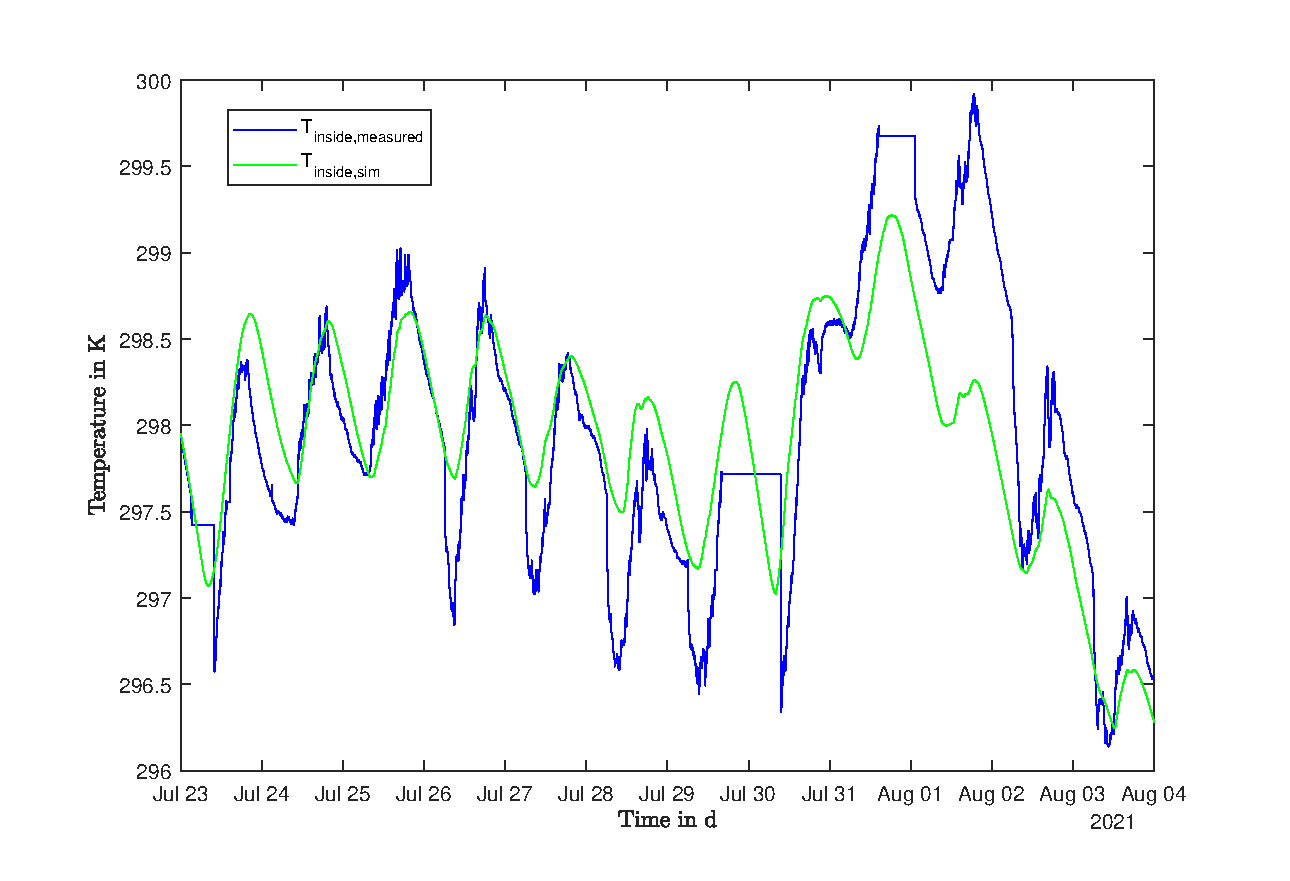
\includegraphics[width=14cm,height=5.5cm]{figure/Training_inside.eps}
           \caption{Training of the building model}
           \label{fig:trainingModel}
    \end{figure}
    \begin{figure}[h]
            \centering
            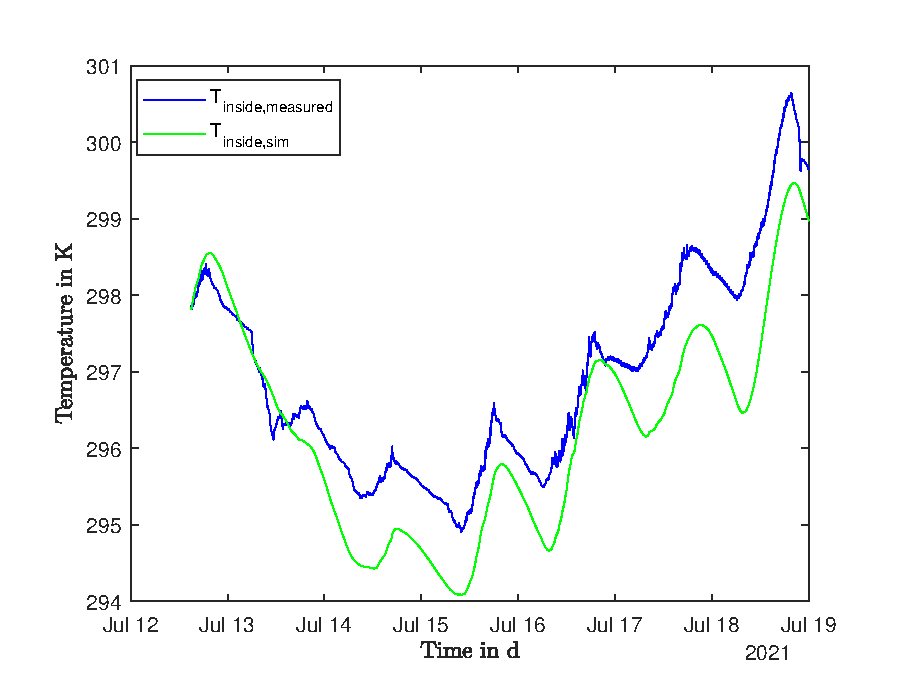
\includegraphics[width=7cm,height=5cm]{figure/Validation_inside.eps}
           \caption{Verification of the building model}
           \label{fig:verificationModel}
    \end{figure}
   \autoref{fig:trainingModel} and \autoref{fig:verificationModel} show the curve of the inside temperature of the simulated and the measured values for the training and verification period. The use of data from an occupied building leads to the difference between the model and the measured inside temperature. The required simple model can not consider random influences such as opening doors and windows, the number of occupants, and the electric consumption in the building. Nevertheless, it can be stated that the model sufficiently well reflects the dynamics of reality. In addition, the Root Mean Square Error (RMSE) \nomenclature[A]{RMSE}{Root Mean Square Error} and the maximum residual ($\mathrm{R}_\text{max}$) is used as verification measure of the model.\newline
    The RMSE is calculated with the quadratic difference of the simulated output $y_\text{sim}$ and the measured output $y_\text {meas}$ as follows \cite{Barnston.1992}: 
    \begin{equation}
        RMSE = \sqrt{\frac{1}{N} \sum \limits_1^N (y_\text{sim} - y_\text {meas})^2}
    \end{equation}
    Here is $N$ the number of measurements or simulated values.
    Based on RSME and $\mathrm{R}_\text{max}$ in Table \ref{tab:RMSEundR}, it can be shown that during the training and verification period, the magnitudes of the RSME and $\mathrm{R}_\text{max}$ are similar. The results of the RMSE and the $\mathrm{R}_\text{max}$ are listed for the two optimised outputs after the training and the verification period.
     \begin{figure}[h]
    \begin{minipage}[t]{0.5\textwidth}
    \vspace{0pt}
        \begin{tabular}{c|c|c|c|c}
             & \multicolumn{2}{|c}{$T_\text{inside}$} & \multicolumn{2}{|c}{$T_\text{envelope}$} \\
             \hline
            RMSE & \cellcolor{gray} 0.52 K & \cellcolor{gray90} 0.84 K & \cellcolor{gray} 0.49 K & \cellcolor{gray90} 0.51 K \\
            $\mathrm{R}_\text{max}$ &\cellcolor{gray} 1.66 K & \cellcolor{gray90} 1.92 K & \cellcolor{gray} 1.21 K & \cellcolor{gray90} 1.00 K
        \end{tabular}
    \end{minipage}
    \hfill
    \begin{minipage}[t]{0.5\textwidth}
    \vspace{0pt}
        \begin{tabular}{c c}
        \\
            &\cellcolor{gray} Training period \\
           &\cellcolor{gray90} Verification period
        \end{tabular}
    \end{minipage}
    \caption{RMSE and $\mathrm{R}_\text{max}$ of the output for training and verification period}
    \label{tab:RMSEundR}
    \end{figure}
    The maximum difference between the training and verification period for the RMSE is 0.32 K and in case of the $\mathrm{R}_\text{max}$ 0.26 K. As a result, the building model is verified. \newline

    \section{The state-space formulation}
    \label{holeModel}
    The white-box model of the water reservoir and the grey-box model of the building behaviour have now been prepared. In the next step, we put them together in the state-space formulation, which we introduced in \autoref{subsection:dynamics}.\newline
    To this end, we separate in control signal $\textbf{u}$ and disturbances $\textbf{d}$. The control signals are the heat flow of the heating system $\dot{Q}_\text{heating}$ and the heat pump in the reference building $\dot{Q}_\text{HP}$. The main disturbances are the weather and, especially for the water reservoir, heat losses. Therefore, the state-space formulation results as follows: 
  \begin{align}
	    \label{eq:ZRD Modell}
	 \left(\begin{array}{c} \frac{d T_\text{inside}}{d t} \\ \frac{d T_\text{envelope}}{d t} \\ \frac{d T_\text{interior}}{d t}\\ \frac{d T_\text{floor}}{d t}\\ \frac{d U_\text{WR}}{d t} \end{array}\right) &= A \left(\begin{array}{c} T_\text{inside} \\ T_\text{envelope} \\ T_\text{interior}\\ T_\text{floor}\\ U_\text{WR} \end{array}\right) + B_\text{1} \left(\begin{array}{c} \dot{Q}_\text{heating} \\ \dot{Q}_\text{HP} \end{array}\right) + B_\text{2} \left(\begin{array}{c} I_\text{sun,inside}\\ I_\text{sun,envelope}\\ T_\text{outside} \\ \dot{Q}_\text{loss} \end{array}\right) \\
	 T_\text{inside} &= C \left(\begin{array}{c} T_\text{inside} \\ T_\text{envelope} \\ T_\text{interior}\\ T_\text{floor}\\ U_\text{WR} \end{array}\right) \nonumber
	\end{align}	
    The complete matrices $A$, $B_\text{1}$, $B_\text{2}$, and $C$ are presented in \autoref{sec:appendix:Matrizen}. We have no pass-through matrices $D_\text{1}$ or $D_\text{2}$ because neither control signals nor disturbances have a direct impact on the output. 